\section{Reflection}

\begin{frame}{Reflection}{missing features}%+fault kode
	\begin{itemize}
		\item
	\end{itemize}
\end{frame}

\begin{frame}{Reflection}{Optimization}
	Minimize communication between server and client
	\begin{itemize}
		\item Search
		\begin{itemize}
			\item .ToList()
		\end{itemize}
		\item Caching
		\begin{itemize}
			\item Save meals locally
			\item Local list of inventory
			\item Better allowance of off-line usage
		\end{itemize}
	\end{itemize}
\end{frame}

\begin{frame}{Reflection}{Evaluation of design}
	\begin{itemize}
		\item Scheduled meal page, update button
		\newline 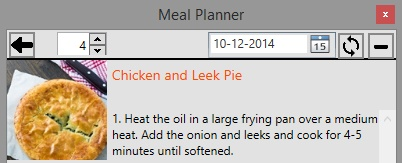
\includegraphics[scale=0.4]{./graphics/datepicker}
		\item Deleting meal
		\newline 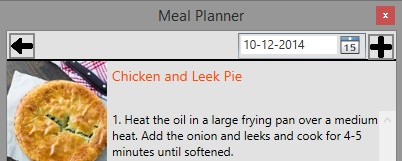
\includegraphics[scale=0.4]{./graphics/datepicker-not-planned}
	\end{itemize}
\end{frame}

\begin{frame}{Reflection}{Requirements}%som er opfyldt/dem som ikke er.
	The two main problems:
	\begin{itemize}
		\item Planning and managing meals
		\item Minimizing food waste
	\end{itemize}	
	Problem based requirements:
	\begin{itemize}
		\item To much food being wasted
		\item Miscalculations happen in groups
		\item Shopping is time consuming
		\item Diets are difficult
		\item Consumers living alone have the most food waste
		\item Consumers living alone have a higher cost per meal
	\end{itemize}

\end{frame}
\begin{frame}{Reflection}{Requirements}%som er opfyldt/dem som ikke er.
The two main problems:
	\begin{itemize} \color{dkgreen}
		\item Planning and managing meals
		\item Minimizing food waste
	\end{itemize}
	Problem based requirements:
	\begin{itemize}
		\item {\color{dkgreen}To much food being wasted}
		\item {\color{red}Miscalculations happen in groups}
		\item {\color{orange}Shopping is time consuming}
		\item {\color{dkgreen}Diets are difficult}
		\item {\color{red}Consumers living alone have the most food waste}
		\item {\color{red}Consumers living alone have a higher cost per meal}
	\end{itemize}
\end{frame}

\begin{frame}{Reflection}{Future improvements}
	\begin{itemize}
		\item Waterfall versus iterative
		\item IDA or focus groups
	\end{itemize}
\end{frame}
